\def\pgfsysdriver{pgfsys-dvipdfm.def}
\documentclass{beamer}
\usepackage{fontspec}
\setmainfont[Mapping=tex-text]{CMU Sans Serif}
\setsansfont[Mapping=tex-text]{CMU Sans Serif}
\setmonofont[Mapping=tex-text]{CMU Typewriter Text}
\usepackage[russian]{babel}
\usetheme{default}
%\setbeameroption{show notes}
\usepackage{listings}
\usepackage{hyperref}
\usepackage{caption}
\usepackage{subcaption}
\usepackage{tabularx}
\usepackage{advdate}
\usepackage{pgfpages}
%\renewcommand\tabularxcolumn[1]{m{#1}}   
\setbeamertemplate{navigation symbols}{}

\setbeameroption{hide notes} % Only slides
%\setbeameroption{show only notes} % Only notes
%\setbeameroption{show notes on second screen=right} % Both
\setbeamertemplate{note page}{\pagecolor{yellow!5}\vfill\insertnote\vfill}

%-------------------------------------------------------------------------------
\setbeamertemplate{headline}{%
\leavevmode%
    \hbox{%
        \begin{beamercolorbox}[wd=\paperwidth,ht=2.25ex,dp=1ex,center]{section in head/foot}%
            \usebeamerfont{section in head/foot}\insertsectionhead
        \end{beamercolorbox}%
    }
}
\makeatletter
\setbeamertemplate{footline}
{
    \leavevmode%
    \hbox{%
        \begin{beamercolorbox}[wd=.333333\paperwidth,ht=2.25ex,dp=1ex,center]{date in head/foot}%
            \usebeamerfont{author in head/foot}\insertshortauthor
        \end{beamercolorbox}%
        \begin{beamercolorbox}[wd=.333333\paperwidth,ht=2.25ex,dp=1ex,center]{date in head/foot}%
            \usebeamerfont{title in head/foot}\insertshorttitle
        \end{beamercolorbox}%
        \begin{beamercolorbox}[wd=.333333\paperwidth,ht=2.25ex,dp=1ex,right]{date in head/foot}%
            \usebeamerfont{date in head/foot}\insertshortdate{}\hspace*{2em}
            \insertframenumber{} / \inserttotalframenumber\hspace*{2ex} 
        \end{beamercolorbox}}%
        \vskip0pt%
    }
\makeatother



%-------------------------------------------------------------------------------
\title[]{Разработка алгоритмов скаффолдинга при помощи дополнительной геномной информации}
\author[Клещин Антон]{Клещин Антон Сергеевич, 16.Б10-мм\\[1ex] 
 {\small Научный руководитель: доц. каф. СП, к.т.н. Литвинов Ю.\,В.\\ Консультанты: доц. каф. СМ, к.ф.-м.н. Коробейников А.\,И. \\ Научный сотрудник Центра алгоритмической биотехнологии СПбГУ Пржибельский А.\,Д.\\ Рецензент: аспирант Мелешко Д.\,А.}}
\institute[]{СПбГУ}
\date{\SetDate[30/05/2020]\today}

\begin{document}

\begin{frame}
\titlepage
  
\note{Добрый день, меня зовут Клещин Антон, и сейчас я расскажу о своей дипломной работе "Разработка алгоритмов скаффолдинга при помощи дополнительной геномной. информации"}
\end{frame}

%-------------------------------------------------------------------------------
% =====================================================================================

\begin{frame}\frametitle{В идеальном мире}
\begin{figure}
    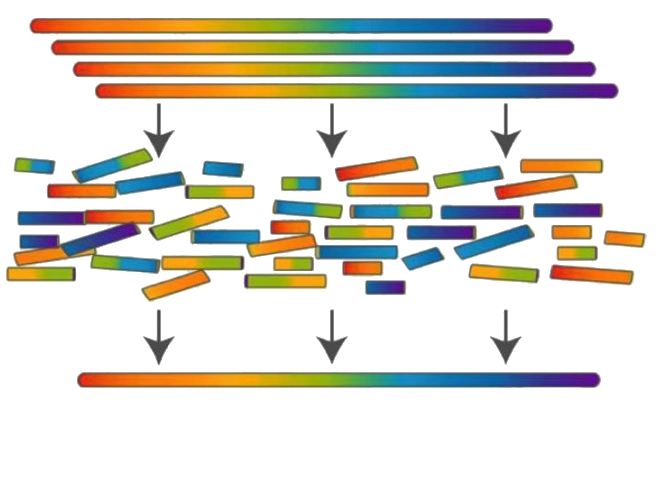
\includegraphics[scale=0.70]{img1.png}
\end{figure}

\note{Несколько слов о том, что такое сборка генома. \\ Есть набор одних и тех же геномов, и их пытаются прочитать и получают огромный набор кусочков --- ридов. В идеале из них геномные сборщики могут восстановить всю ДНК.}
\end{frame}

% =====================================================================================

\begin{frame}\frametitle{В реальности}
\only<1> {
\begin{figure}
    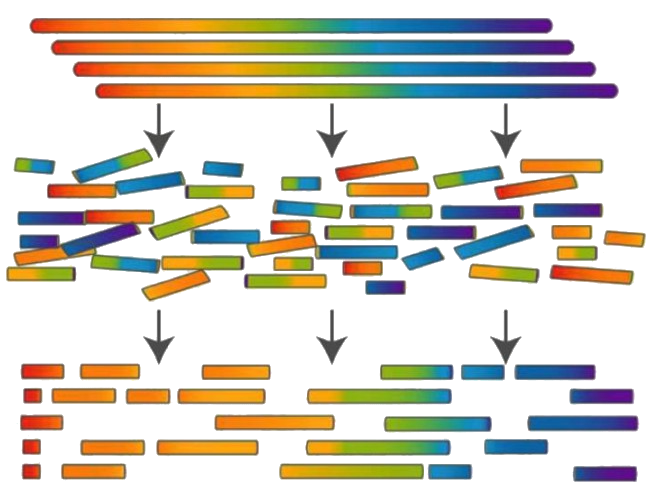
\includegraphics[scale=0.70]{img2.png}
\end{figure}
\note{Но на деле удаётся восстановить только некоторые фрагменты. Они называются контигами. Если известен порядок двух контигов и расстояние между ними, то это называется скаффолд. Референсным геномом называется эталонный геном для данного вида организма. }
}
\only<2> {
\begin{figure}
    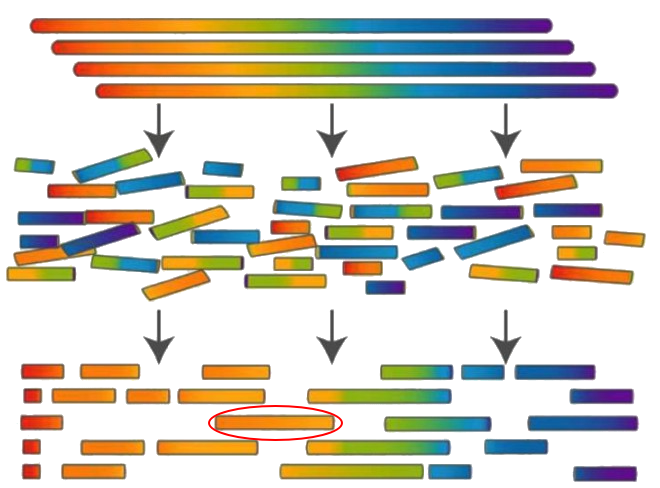
\includegraphics[scale=0.70]{img3.png}
\end{figure}
\note{Основная идея работы состоит в том, что если кто-то скажет, что в геноме должна быть последовательность, похожая на ту, что обведена красным, то можно посмотреть на два контига выше, понять, что их края достаточно похожи на края выделенного фрагмента и затем объединить все три в один.}
}

\end{frame}

% =====================================================================================


\begin{frame}\frametitle{Мотивация}
\begin{itemize}
    \item Переиспользование накопленных результатов
    \item Использование результатов сторонних ассемблеров
    \item Использование похожих геномов
    \item Упрощение метагеномной сборки использованием референсных геномов
\end{itemize}
\note{Изначально всё затевалось для геномного ассемблера SPAdes под эгидой "переиспользования накопленных результатов'', потому что есть исследователи, которым это нужно, а использование контигов под видом длинных ридов их не устраивало.\\ \mbox{} \\
Также есть биологи, которые используют другой ассемблер для сборки из специального типа ридов, а затем используют его результат как дополнительную информацию в SPAdes.\\ \mbox{} \\
Также есть два скорее теоретических применения: \\
Во-первых, это использование похожих геномов, таких как другие штаммы бактерий. \\
Во-вторых, это применение в метагеномике. В метагеномной сборке присутствуют риды не одного организма, а сразу множества. И если есть информация о том, какие организмы могут присутствовать в этом множестве, то можно использовать их референсные геномы для упрощения всей сборки.
}
\end{frame}

% =====================================================================================

\begin{frame}\frametitle{Постановка задачи}
Цель --- добавление поддержки контигов в качестве входных данных для геномного ассемблера SPAdes
\begin{itemize}
    \item Разработка алгоритма скаффолдинга, использующего
контиги
    \item Реализация расширения для геномного ассемблера SPAdes
    \item Тестирование алгоритма на известных геномах
\end{itemize}
\note{Цель данной работы --- добавление поддержки контигов в качестве входных данных для геномного ассемблера SPAdes. Для этого нужно было разработать алгоритм, использующий контиги, реализовать его и протестировать.}
\end{frame}

% =====================================================================================

\begin{frame}\frametitle{Алгоритм}
\begin{itemize}
	\item Построение графа сборки
		\begin{itemize}
			\item Короткие риды
			\item Контиги
		\end{itemize}
	\item Упрощение графа
	\item Выравнивание контигов на граф
	\item Выращивание путей
		\begin{itemize}
			\item Точное совпадение с путями выравненных контигов
			\item Неточное совпадение
		\end{itemize}
	\item Постобработка 
\end{itemize}
\note{Сборка в SPAdes основывается на построении графа сборки --- на его рёбрах находятся последовательности нуклеотидов, а путь в нём образует контиг. Поэтому основная идея алгоритма заключается в том, чтобы сначала выравнять входные контиги на граф сборки, то есть получить набор путей, образующих эти контиги (или их части), а затем использовать их как вспомогательные на этапе выращивания путей. На этом этапе берутся некоторые начальные пути графа и затем к их концам пытаются присоединять ребра.\\ \mbox{} \\
Но выравнивание на граф сборки --- это очень вычислительнозатратная операция, поэтому происходит она не напрямую. Сначала контиги используются для построения графа сборки. Затем во время упрощения графа все рёбра, содержащие ошибки, удалятся, но при этом похожие рёбра объединятся. Теперь во время выравнивания контигов можно сравниваться не просто с подстроками рёбер, а с их известными возможными вариациями. Благодаря этому выравнивание на граф происходит в сотни раз быстрее.
}
\end{frame}

% =====================================================================================

\begin{frame}\frametitle{Архитектура}
\begin{figure}
    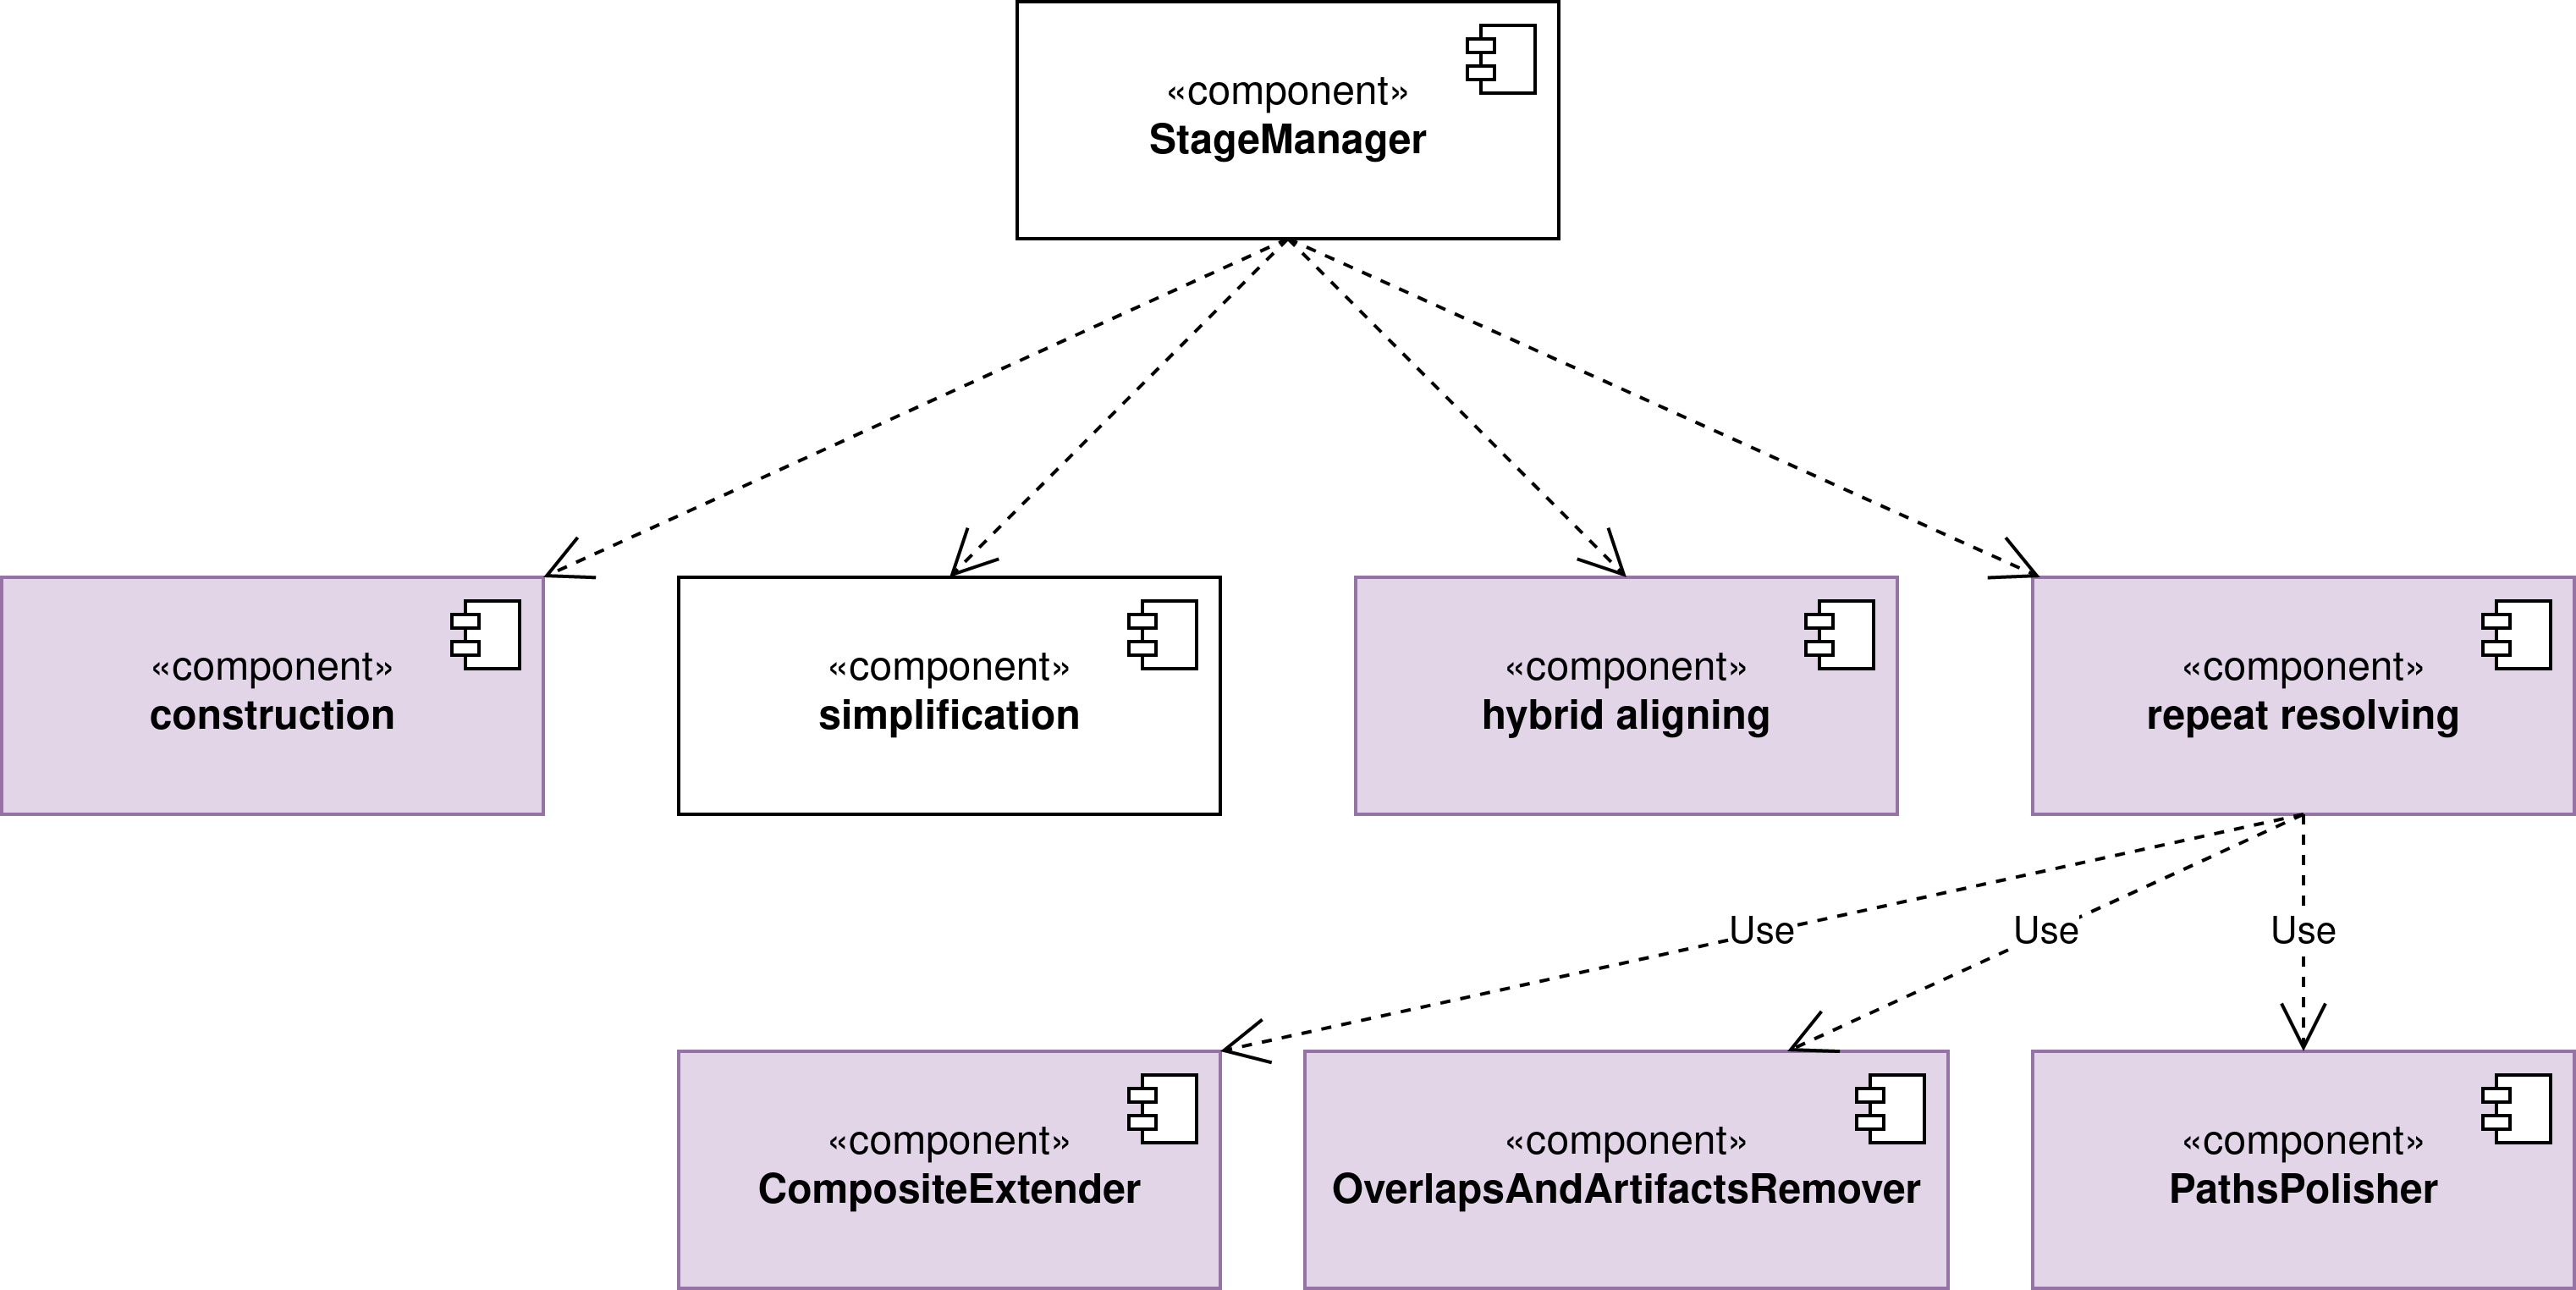
\includegraphics[width=\textwidth]{components.png}
\end{figure}
\note{На этом слайде изображены этапы сборки, упомянутые в алгоритме. Фиолетовым выделены изменённые компоненты. Hybrid alining отвечает за выравнивание на граф, CompositeExtender занимается выращиванием путей, а OverlapsAndArtifactsRemover и PathPolisher выполняют постобработку путей. Остановимся подробнее на двух этапах.}
\end{frame}

% =====================================================================================

\begin{frame}\frametitle{Архитектура}
\begin{figure}
    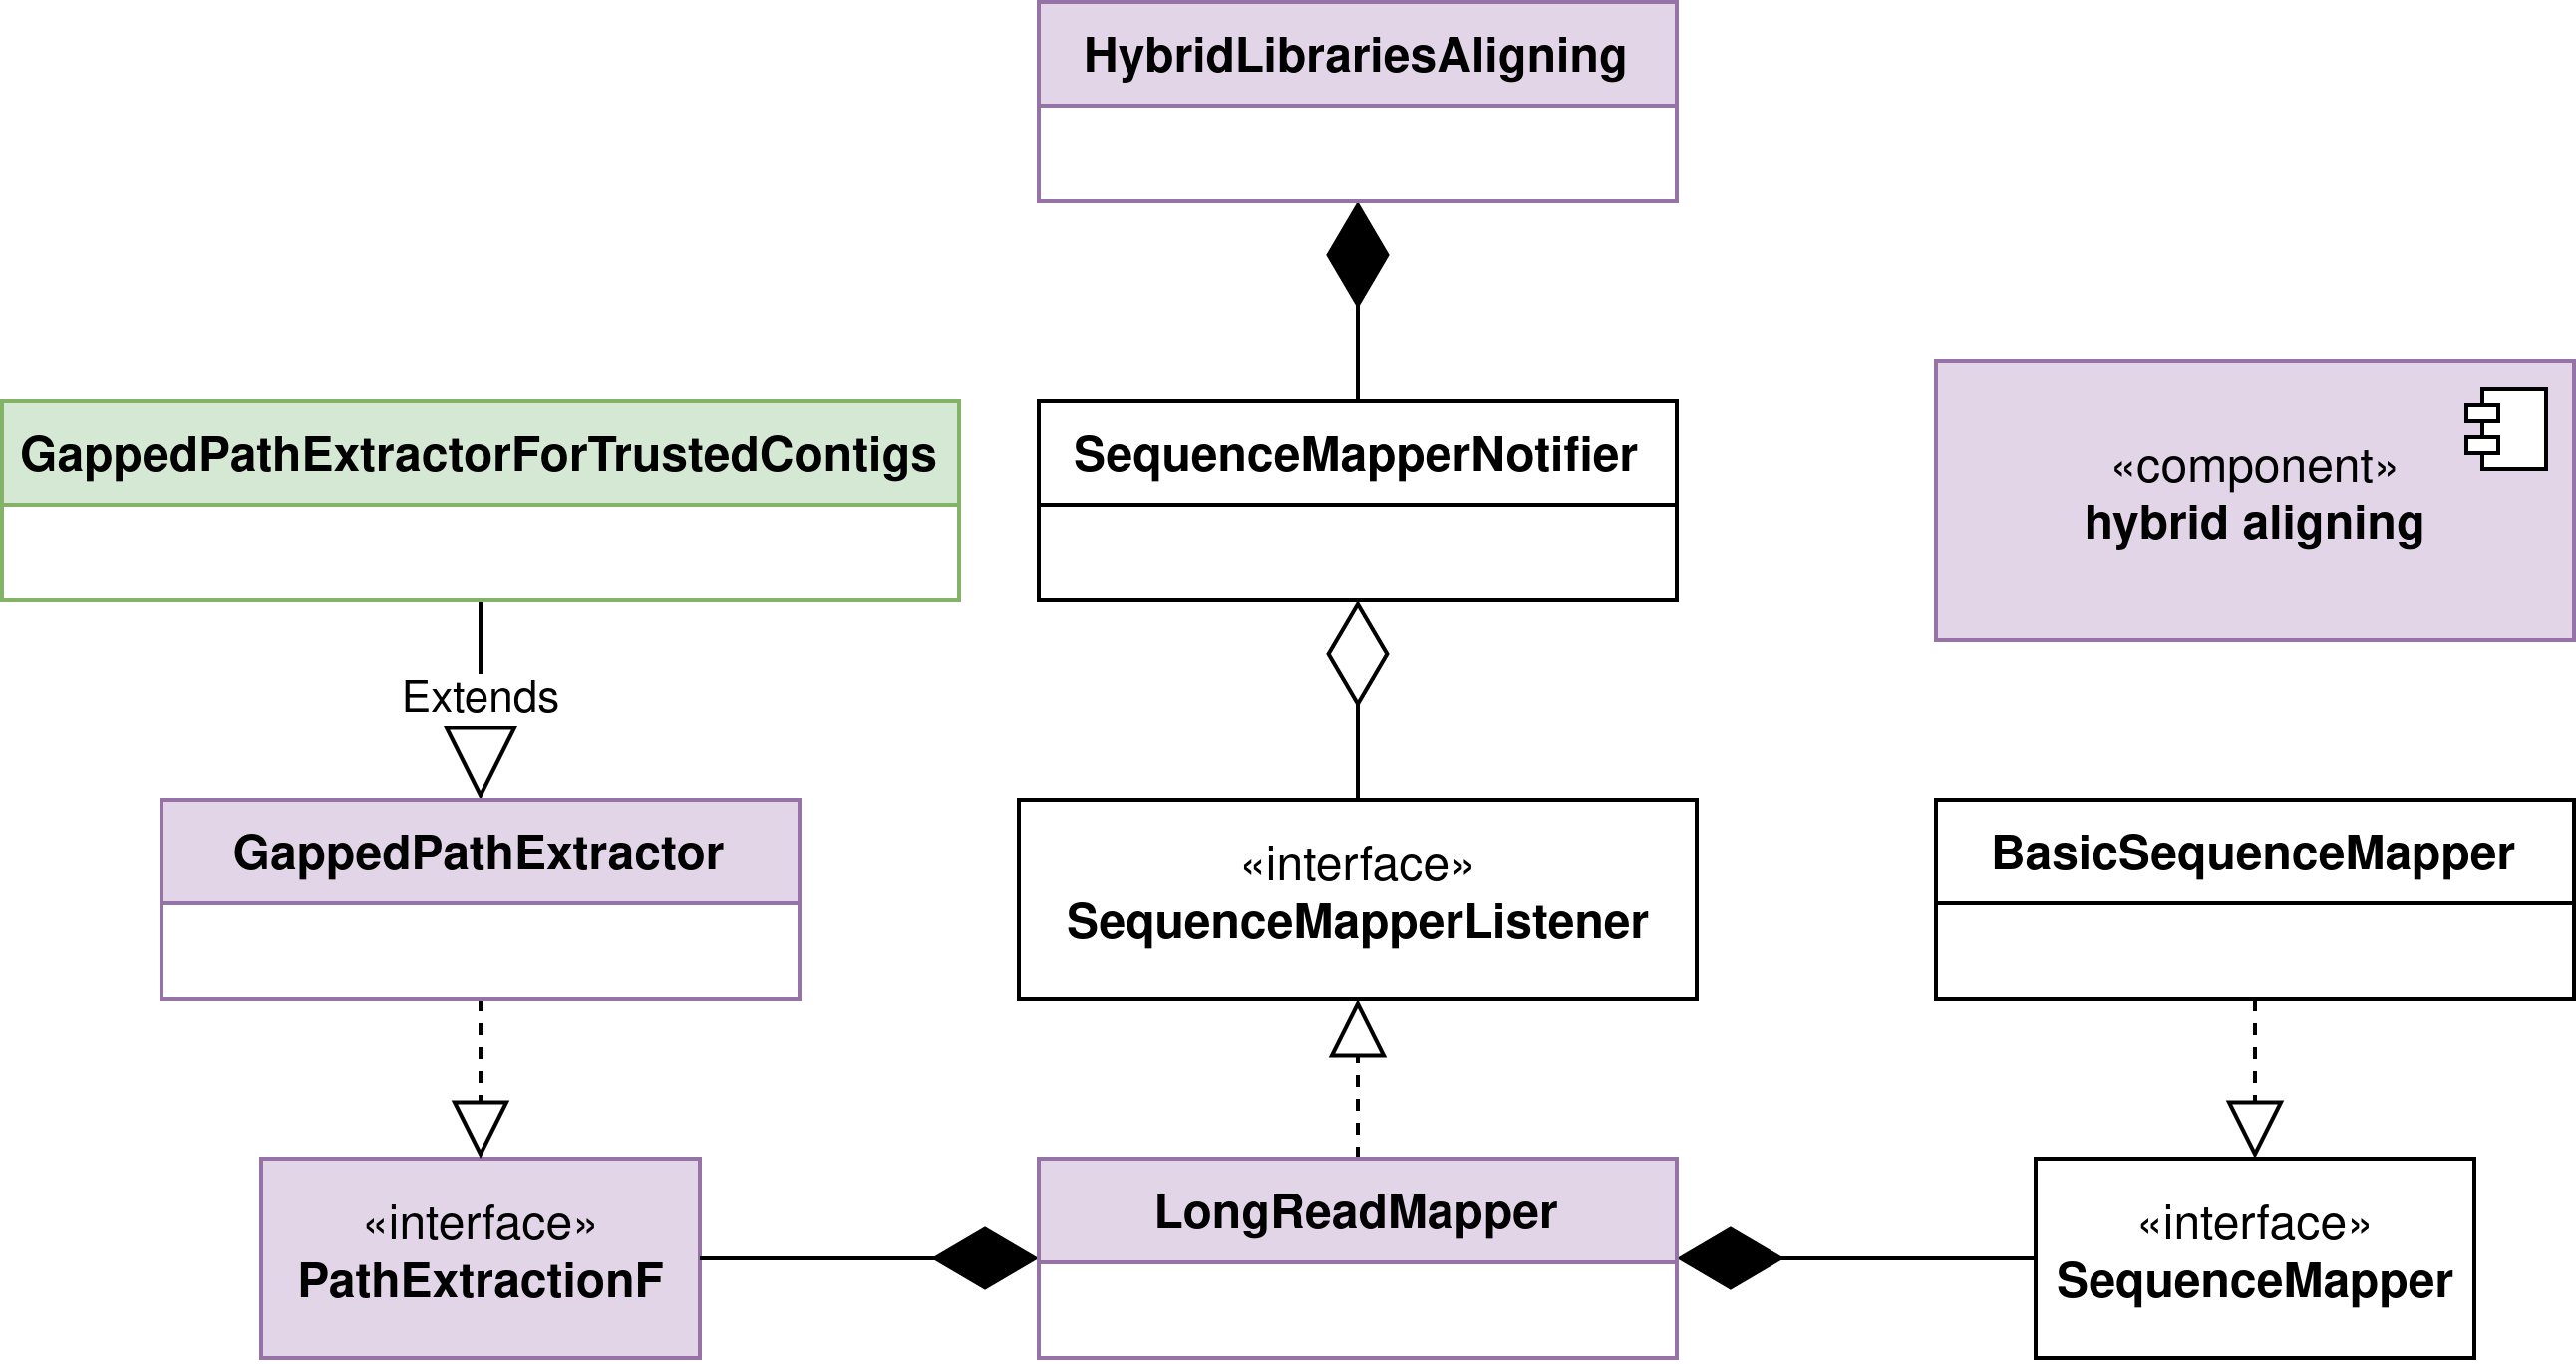
\includegraphics[width=\textwidth]{mapper.png}
\end{figure}
\note{Первым будет выравнивание на граф. Зелёным выделен класс, написанный с нуля. \\ \mbox{} \\
Этап выравнивания входных данных на граф сборки начинается с класса HybridLibrariesAligning. Он занимается подготовительной работой, создавая и конфигурируя классы, занимающиеся выравниванием соответствующих типов ридов, а затем связывает их с потоками входных данных через систему уведомлений SequenceMapperNotifier. После этого он начинает многопоточную обработку данных.
\\ \mbox{} \\
Для выравнивания контигов используется класс LongReadMapper, который параметризуется двумя алгоритмами: SequenceMapper и PathExtractionF. Первый занимается сопоставлением контига фрагментам рёбер графа. Эти фрагменты затем собираются, фильтруются, объединяются в рёбра, а затем и в пути вторым алгоритмом.
}
\end{frame}

% =====================================================================================

\begin{frame}\frametitle{Архитектура}
\begin{figure}
    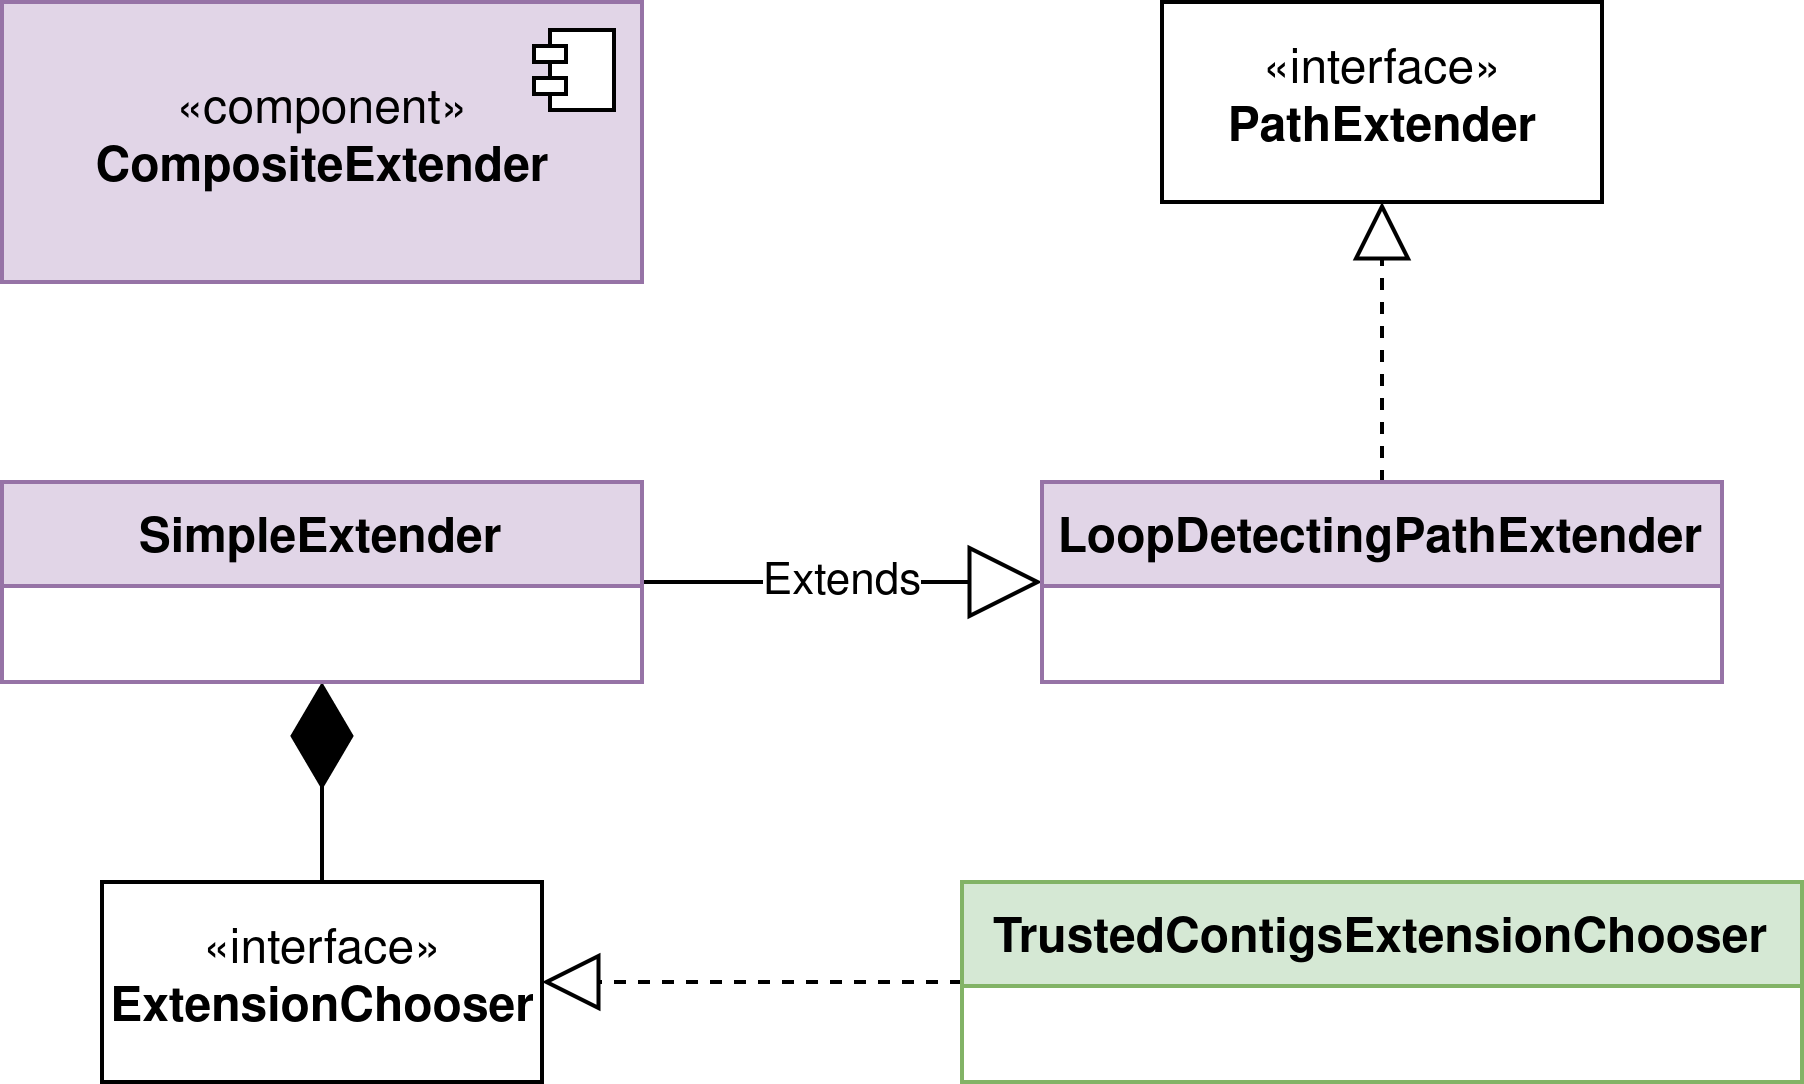
\includegraphics[width=0.7\textwidth]{extenders.png}
\end{figure}
\note{
На стадии выращивания путей создаётся набор PathExtender'ов в соответствии со входными данными. Каждый PathExtender позволяет продолжить переданный ему путь на одно ребро. С помощью CompositeExtender все созданные PathExtender'ы применяются последовательно в соответствии с некоторым приоритетом, пока одному из них не удастся продолжить путь. 
\\ \mbox{} \\
Одной из реализаций PathExtender является SimpleExtender. Он параметризуется алгоритмом ExtensionChooser, который по пути определяет, какие рёбра возможны для его продолжения. В случае если продолжение единственно, методами LoopDetectingPathExtender проверяется, можно ли добавить его.
}
\end{frame}

% =====================================================================================

\begin{frame}\frametitle{Метрики}

\begin{itemize}
	\item Количество больших контигов
	\item Количество структурных ошибок
\end{itemize}
\note{В данной работе были использованы четыре метрики, но для демонстрации результатов достаточно двух из них. Это количество больших контигов и количество структурных ошибок.
\\ \mbox{} \\
Уменьшение числа больших контигов означает, что удалось объединить несколько других больших контигов в один. Поэтому чем их меньше, тем лучше.
\\ \mbox{} \\
Структурные ошибки --- это места в контигах, в которых соединения быть не должно. То есть соединения есть в контиге, но отсутствуют в референсном геноме.
}
\end{frame}

% =====================================================================================

\begin{frame}\frametitle{Тестирование}
\begin{figure}
    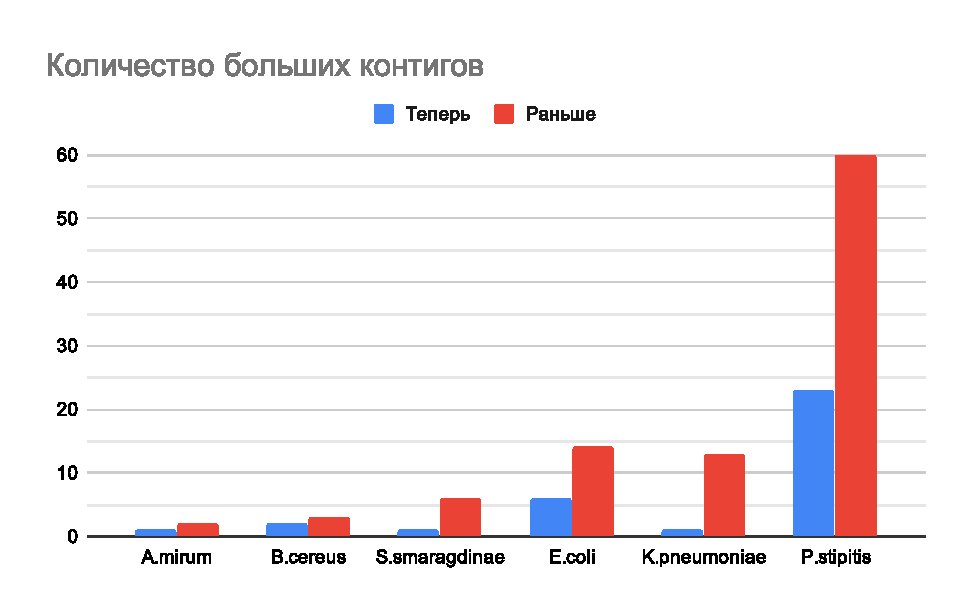
\includegraphics[width=\textwidth]{contigs.eps}
\end{figure}
\note{В SPAdes уже существовала возможность использования контигов в качестве входных данных, но она фактически являлась набором алгоритмов для длинных ридов, а не контигов. Так как контиги можно рассматривать как длинные риды, то этот подход работал, но, очевидно, далеко не самым оптимальным образом.
\\ \mbox{} \\
На этом слайде представлены результаты некоторых сборок одиночных организмов. В качестве входных контигов использовались референсные геномы.
\\ \mbox{} \\
Первые пять элементов являются бактериями, а последний --- грибом с девятью хромосомами. У грибов геном значительно сложнее, поэтому граф сборки получается запутаннее, и поэтому такое резкое ухудшение результатов по сравнению с остальными геномами вполне ожидаемо.
}
\end{frame}

% =====================================================================================

\begin{frame}\frametitle{Тестирование}
\begin{figure}
    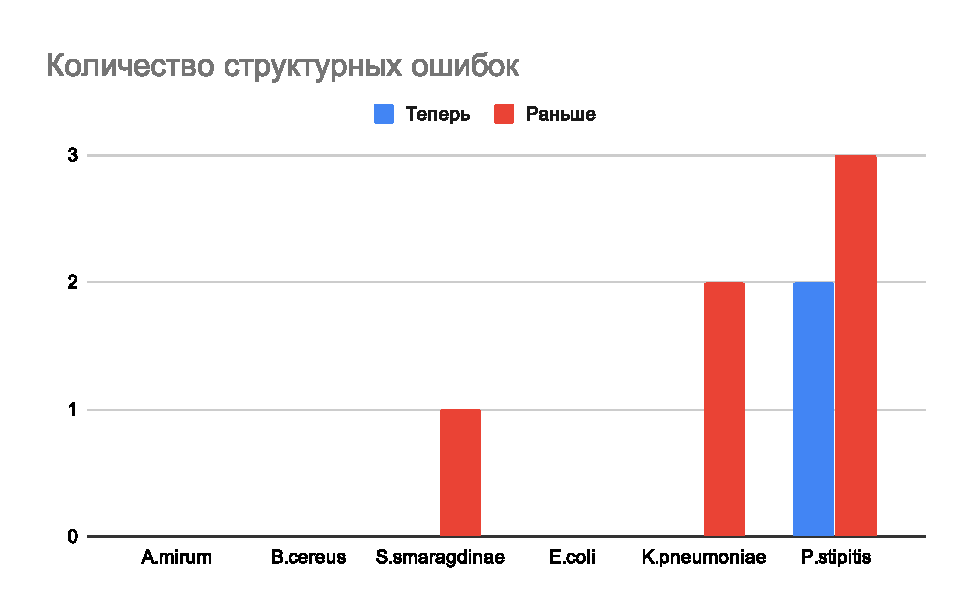
\includegraphics[width=\textwidth]{misassemblies.eps}
\end{figure}
\note{Из этого графика видно, что количество структурных ошибок также уменьшилось.}
\end{frame}

% =====================================================================================

\begin{frame}\frametitle{Тестирование, Flye}
\begin{figure}
    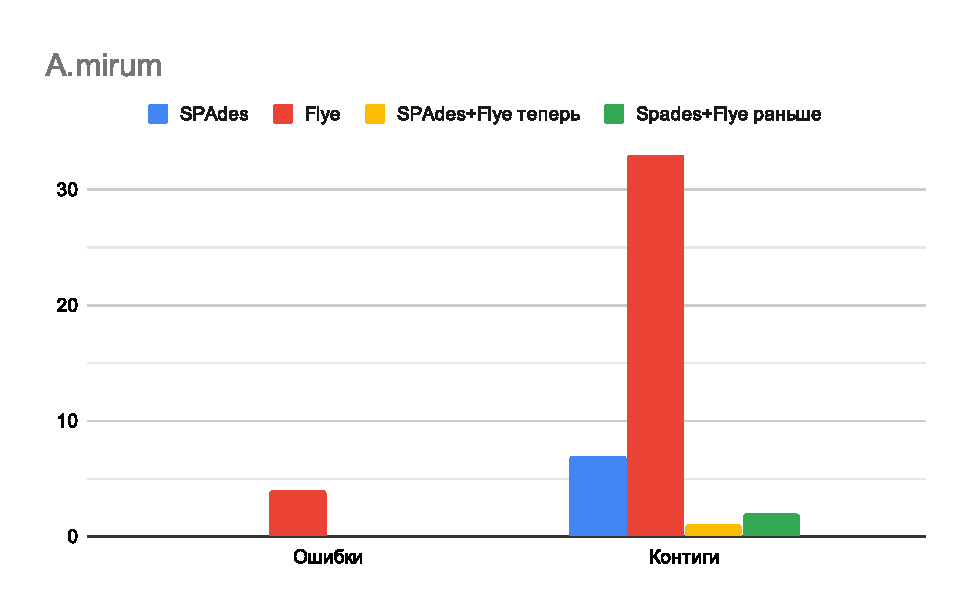
\includegraphics[width=\textwidth]{A.mirum.eps}
\end{figure}
\note{В начале презентации я упоминал биологов, которые используют сторонний ассемблер. Они используют Flye для сборки из специфических ридов, получают не очень хороший результат сборки, который дальше используют в SPAdes уже со всеми доступными им ридами. Здесь результаты не говорят о плохой работе Flye, ему просто дают такие входные данные, что лучше сделать сложно.}
\end{frame}

% =====================================================================================

\begin{frame}\frametitle{Тестирование, метагеном}
\begin{figure}
    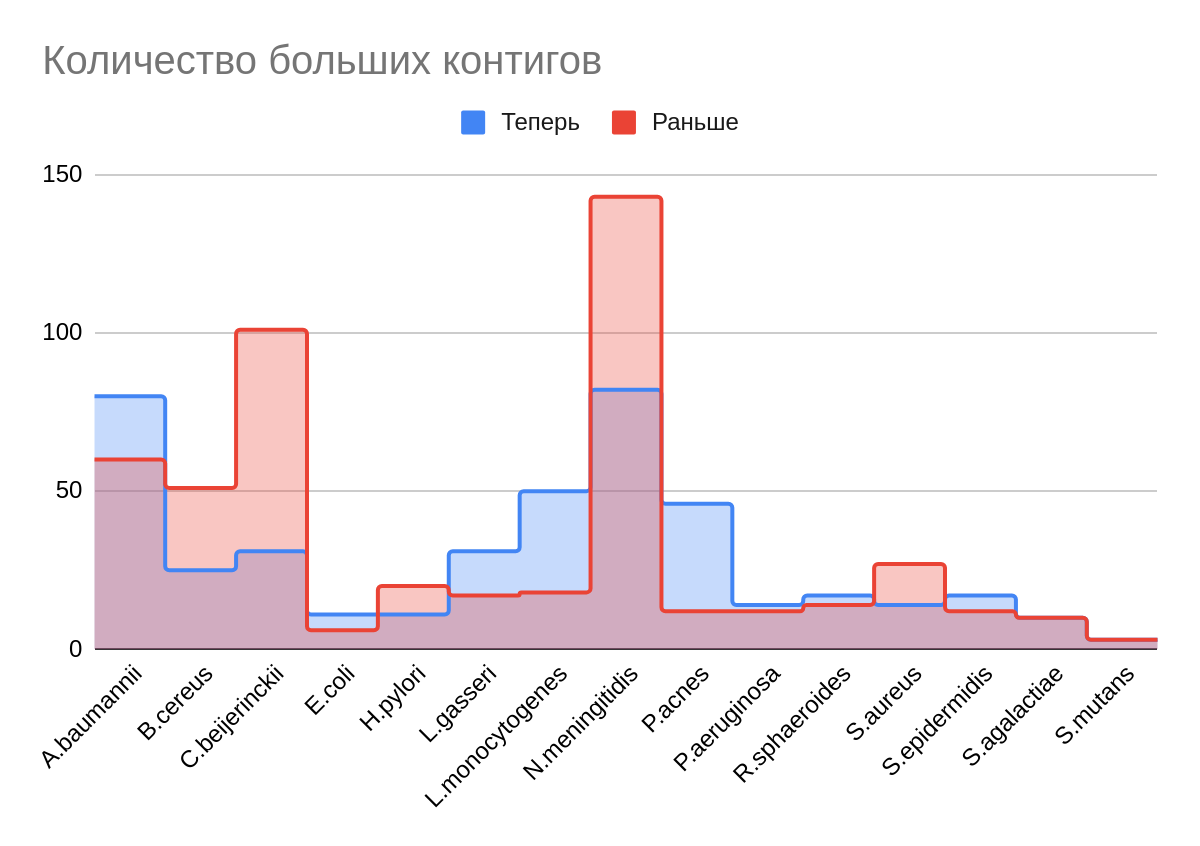
\includegraphics[width=\textwidth]{mock_contigs.png}
\end{figure}
\note{На этом слайде показаны результаты тестирования на метагеномной сборке. Риды всех бактерий с графика передавались в ассемблер одной кучей. В качестве контигов передавались референсные геномы бактерий. \\ \mbox{} \\
Видно, что для некоторых бактерий количество больших контигов возросло, то есть результаты по этой метрике ухудшились. }
\end{frame}

% =====================================================================================

\begin{frame}\frametitle{Тестирование, метагеном}
\begin{figure}
    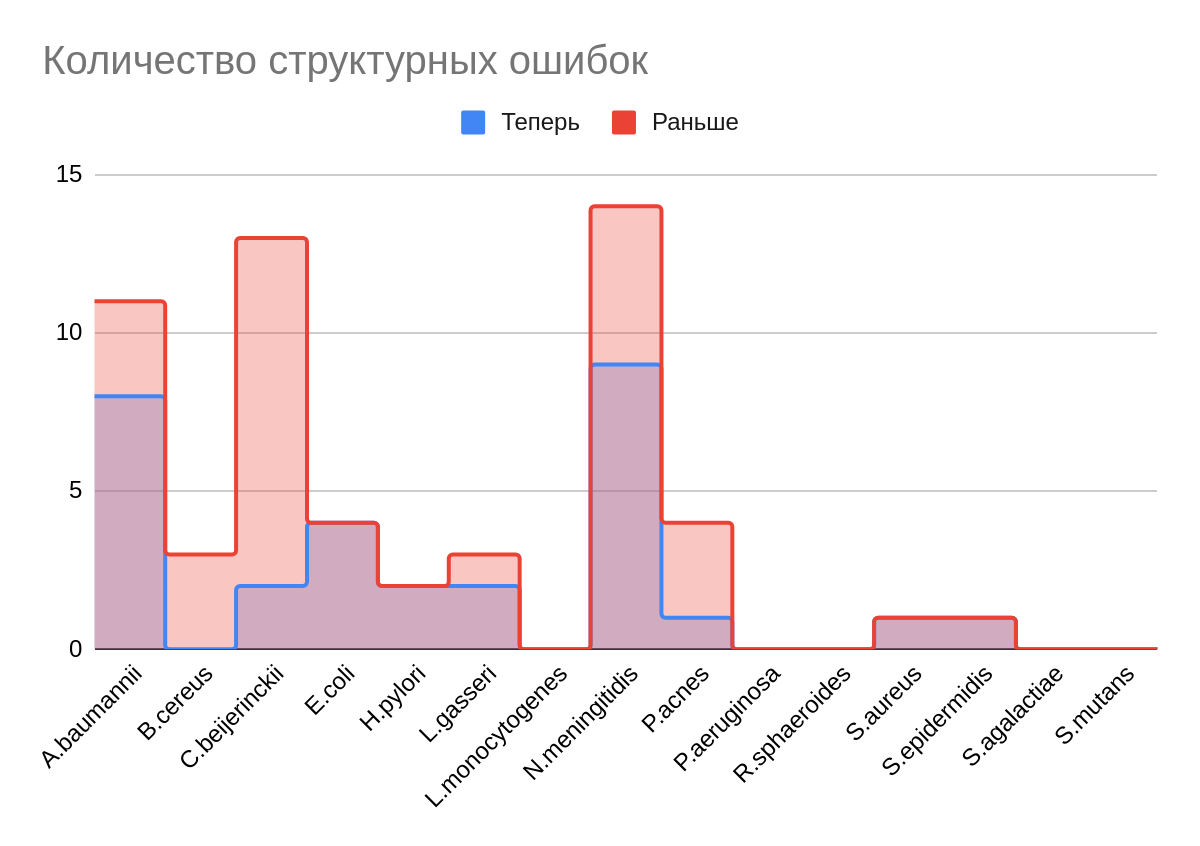
\includegraphics[width=\textwidth]{mock_mis.png}
\end{figure}
\note{Но здесь главным достижением является то, что удалось существенно уменьшить количество структурных ошибок. Это важнее, потому что биологу найти ошибку в сборке значительно сложнее, чем объединить контиги. }
\end{frame}

% =====================================================================================

\begin{frame}\frametitle{Заключение}
\begin{itemize}
    \item Разработан алгоритм скаффолдинга, использующего
контиги
	\begin{itemize}
		\item Алгоритм выравнивает контиги на граф сборки, а затем использует полученные пути при разрешении повторов
	\end{itemize}
    \item Реализовано расширение для геномного ассемблера SPAdes
	\begin{itemize}
		\item Реализовано на языке C++
		\item Расширение позволяет эффективно использовать контиги в качестве входных данных
		\item \begin{sloppypar} Исходный код SPAdes доступен по ссылке: \mbox{\url{https://github.com/ablab/spades/}}.\end{sloppypar}
	\end{itemize}
    \item Алгоритм протестирован на известных геномах
	\begin{itemize}
		\item Протестировано на сборках одиночных геномов с высоким и низким качеством входных контигов, а также на метагеномной сборке
		\item Теперь соединяется больше контигов с меньшим количеством ошибок по сравнению с предыдущим модулем SPAdes
	\end{itemize}
\end{itemize}
\note{Итак, в ходе данной работы были достигнуты следующие результаты. Разработан алгоритм скаффолдинга, использующий контиги. Реализовано расширение для геномного ассемблера SPAdes на языке C++. Оно войдёт в состав следующего релиза. А также проведено тестирование на известных геномах, и оно показало, что теперь соединяется больше контигов с меньшим количеством ошибок по сравнению с предыдущим модулем SPAdes.}
\end{frame}

% =====================================================================================

\end{document}